\section{The Simulation}
\label{sec:simulation}

\begin{table}[!tbhp]
	\centering
	\begin{tabular}{ll}
		\toprule
		Parameter & Expected value \\ \midrule
		% Screen width & \SI{1}{\meter} \\
		% Screen height & \SI{65}{\milli\meter} \\
		% % FOV 1.149
		% Horizontal pixels & 1850 \\
		% % optical point spread function set to 0?
		% % width of x sensor? \SI{25e-3}{\metre}
		% Screen efficiency & \SI{5000}{photons\per electron}\\
		% Camera acceptance & \num{1.5e-5} \\
		Emittance \(\epsilon\) & \SI{1e-6}{\meter\radian} \\
		\(\beta\) & 1 \\ % TODO units
		\(\alpha\) & 0.5 \\ % TODO units
		Mean energy \(\bar E\) & \SI{1.3}{\giga\electronvolt} \\
		Energy spread \(\sigma_E\) & \SI{0.4}{\giga\electronvolt} \\
		N. electrons \(N_{e^-}\) & \num{1e9} \\
		% \(N_{e^-}\) & \num{4e8} \\
		Bg. photons & \SI{3.415e4}{\per\meter\squared} \\
		% Thermal electrons \(N_{e^-_\text{thermal}}\) & \SI{0.016}{\per\second} \\
		\bottomrule
	\end{tabular}
	\caption{
		The expected values for many experimental parameters have been
		calculated. It should be noted that these values are missing error
		values. It can be assumed that the error on each value can be given by
		half the least significant digit.
	}
	\label{tab:expected}
\end{table}

The simulation of this experiment was split into three parts: the simulation of
the beam, the simulation of the effects of the background and camera, and the
reconstruction of the beam to measure the parameters of the beam.
% the following is bs
% It is designed such that each part of the code is able to act independently.

\subsection{The Electron Beam}

Given enough computing power and time, the simulation of the beam from, the end
of the plasma cell, passing through two quadrupoles and through a dipole could
have been done on BDSIM~\cite{agapov2009bdsim}, a
Geant4~\cite{agostinelli2003geant4} toolkit for simulating radiation traveling
through an accelerator. This software package simulates a each particle
individually, updating it's position and velocity at each step through the
accelerator by applying the effect of forces from all fields within the
accelerator.  For beams consisting of \num{\sim e9} particles, tracking each
particle individually as they travel down the beam line would take enormous
amounts of time and available computing power, and as many simulations were
required to be performed this would have been impractical for obtaining any
reasonable amount of data.

A new program was written, taking advantage of beam matrices to describe the
beam as a whole. The goal of the first part of this program is to simulate the
intensity of the incident beam at each pixel on the screen.

\subsubsection{BDSIM calibration}

\begin{figure*}[!tbhp]
	\centering
	% 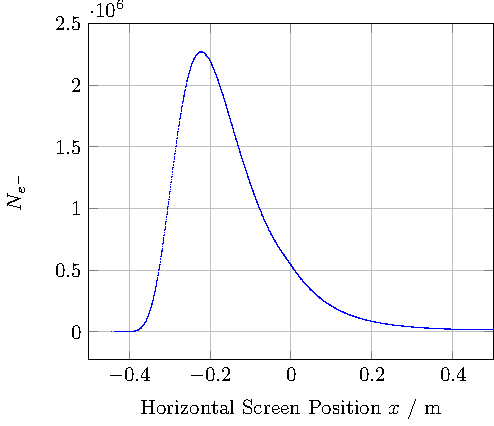
\includegraphics[width=1\linewidth]{./figures/edist.pdf}
	\begin{subfigure}[t]{\columnwidth}
		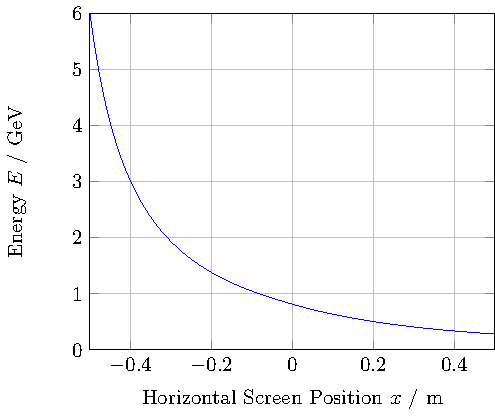
\includegraphics{./figures/eofx.pdf}
		\caption{
			Electron energies corresponding to each vertical pixel strip.
		}
		\label{fig:eofx}
	\end{subfigure}\hfill~
	\begin{subfigure}[t]{\columnwidth}
		% 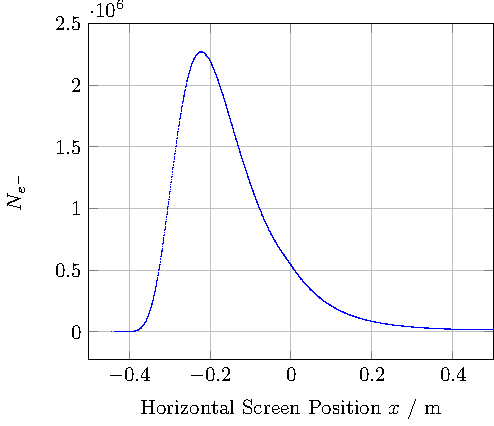
\includegraphics[width=1\linewidth]{./figures/edist.pdf}
		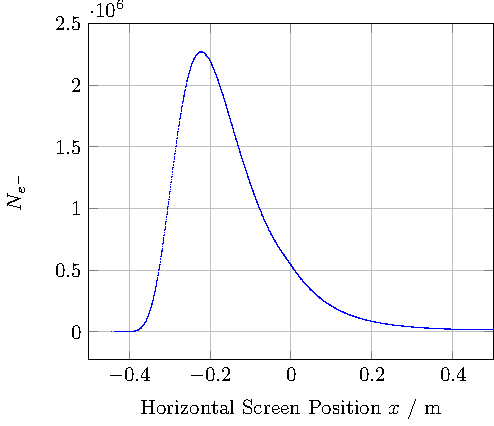
\includegraphics{./figures/edist.pdf}
		\caption{
			The number of electrons expected to hit the screen at each \(x\)
			position for \(E=\SI{1.3}{\giga\electronvolt}\) and
			\(\sigma_E=\SI{0.4}{\giga\electronvolt}\).
			% other experimental parameters are set to their expected values.
		}
		\label{fig:edist}
	\end{subfigure}
	\caption{
		The functions \(E(x)\) and \(N_{e^-}(x)\) extracted from the BDSIM
		calibration output data. These functions are used to calculate the
		horizontal spread of the electrons across the screen.
	}
\end{figure*}

The effect of the quadrupole and the dipole are dependant on the energy of the
individual electrons in the beam. This 

% TODO why we needed the BDSIM runs at all

% So binning each generated electron depending
% on it's energy and applying the transport matrix to each bin of electrons may
% seem to be the obvious next step. However, it is actually more useful to
% % or to greatly simplify the simulation?
% work backwards, starting with each vertical strip of pixels and calculating the
% number of electrons with energy corresponding to the energy range expected to hit
% that strip of the screen.

% The dipole spreads the beam across the screen splitting it into multiple beams
% each with equal energies. The spreading of this beam is discretised, depending on
% the This spreading is neither linear or quadratic and in
% fact is 

So to calculate the density of an electrons along with their energies as a
function of the horizontal screen position a number of BDSIM simulations were
run. \num{e5} electrons where fired individually down the simulated AWAKE beam
line. These electrons had a square energy distribution from \SIrange{0}{10}
{\tera\electronvolt}, and had a Gaussian spacial distribution with \(\sigma_x =
\sigma_y = \SI{6}{\milli\meter}\), and no transverse momentum hence zero
emittance. This large energy range was chosen as to encompass the entire energy
range that would hit the screen. The dipole was set to it's highest setting of
\SI{650}{\ampere} to achieve the maximum spread of the beam on the screen.
% TODO why use no emittance beams for calibration 
These were used to plot the functions in Figures~\ref{fig:eofx} and
\ref{fig:edist}.

% Since the effect of the dipole on the beam depends on the energy of each
% individual particle, the evolution of the beam through the dipole cannot be
% calculated reasonably using beam matrices. So, to simulate the dipole, 

\subsubsection{Deriving the Beam Size Function}

The dipole spreads the beam such that the
electrons in each vertical strip of pixels can be grouped together and their
energy approximated to be equal, as the energy spread in each strip will always
be less than \SI{0.5}{\percent}. This was calculated from Figure~\ref{fig:eofx}
by dividing the difference in energies between adjacent strips by the energy
value at that strip for all strips and the maximum value was \SI{0.5}{\percent}.



The root mean square of the vertical beam size on the screen can be extracted
from the resultant beam matrix \(\sigma_1\).  To arrive at this beam matrix, the
transport matrix \(\mathcal{M}\) is applied to the initial beam matrix
\(\sigma_0\). The transport matrix is the product of the transport matrices for
each component of the spectrometer:

\begin{equation}
	\mathcal{M} = \mathcal{M}_d(d) \cdot \mathcal{M}_{QD}(l_2) \cdot \mathcal{M}_d(g_2)
				  \cdot \mathcal{M}_{QF}(l_1) \cdot \mathcal{M}_d(g_1)
\end{equation}

% TODO why is the first gap not taken into account?
% how are the quadrupole lengths calculated?

The beam matrix element \(\sigma_{11} = \langle y \rangle^2 = \epsilon\beta\)

Applying the matrix multiplication results in the vertical beam size as a
function of the horizontal screen position:

\begin{equation}
	\sigma_y^2 = \sigma_{1,11} = C^2(x)\sigma_{0,11} + 2C(x)S(x)\sigma_{0,12}
								+ S^2(x)\sigma_{0,22}
\end{equation}

% \begin{align*}
% 	\bm{\sigma}_1 &=
% 	\epsilon
% 	\begin{pmatrix}
% 		\beta & -\alpha \\
% 		-\alpha & \gamma
% 	\end{pmatrix} =
% 	\mathcal{M}\;\bm{\sigma}_0\;\mathcal{M}^T, \quad
% 	% \text{where}\quad
% 	\epsilon = \sqrt{\det{\bm{\sigma}}}, \quad
% 	\beta\gamma-\alpha^2=1, \quad
% 	\tan2\varphi = \tfrac{2\alpha}{\gamma-\beta}
% 	\\[1em] %
% 	\mathcal{M} &= \underbrace{
% 	\begin{pmatrix}
% 		1 & d \\
% 		0 & 1
% 	\end{pmatrix}}_\text{drift}
% 	\cdot
% 	\underbrace{
% 	\begin{pmatrix}
% 		\cos\varphi_1 & \tfrac{\sin\varphi_1}{\sqrt{k_1}} \\
% 		-\sqrt{k_1}\sin\varphi_1 & \cos\varphi_1
% 	\end{pmatrix}}_\text{vertically focusing quadrupole}
% 	\cdot
% 	\underbrace{
% 	\begin{pmatrix}
% 		1 & g_2 \\
% 		0 & 1
% 	\end{pmatrix}}_\text{gap}
% 	\cdot
% 	\underbrace{
% 	\begin{pmatrix}
% 		\cosh\varphi_2 & \tfrac{\sinh\varphi_2}{\sqrt{|k_2|}} \\
% 		-\sqrt{k_2}\sinh\varphi_2 & \cosh\varphi_2
% 	\end{pmatrix}}_\text{horizontally focusing quadrupole}
% 	\cdot
% 	\underbrace{
% 	\begin{pmatrix}
% 		1 & g_1 \\
% 		0 & 1
% 	\end{pmatrix}}_\text{gap}
% \end{align*}


After generating, a two dimensional histogram representing the number of
electrons hitting the screen at each pixel the goal is to simulate the
effectiveness of the equipment and translate this number to represent the raw
signal that will be read off for each pixel.

\subsection{Backgrounds}

How good the measurement of the emittance is, is most dependant on the magnitude
of the multiple sources of backgrounds as well as the reliability of the
equipment. The following sources of error were taken into account: the
efficiency of the scintillator screen, the acceptance of the camera due to it's
distance from the scintillator screen, the background photon density, the
emittance of photoelectrons in the camera, the thermal noise in the camera, the
amplification by the microchannel plate (MCP) and the readout noise.  Each
source of noise is added to each pixel independently.

% TODO ask about the acceptance value.
% do we assume scintillator emits photons evenly?
% how far is the camera from the screen - I should know this
% what is the acceptance of the camera?
% where does the value 1e5*64/80 come for the background photon density?
% where do we assume the background photon density comes from

% TODO cite 5000
The first two error sources, the scintillator screen and the camera acceptance,
both scale the signal. So for each electron that hits the screen, it is
expected that an average of \num{5000} photons are to be emitted. The
camera acceptance, is the ratio of photons that the camera registers to the
number of photons emitted by the scintillator, with a value of \num{1.5e-5}.
After the addition of these two effects, the camera is expected to receive
\SI{7.5}{\percent} of the original electron signal. The expected value for the
number of photons incident on the camera due to the beam electrons is a Poisson
random number.

It is assumed that there is a uniform distribution of photons incident on the
camera. The density of these electrons is expected to be
\SI{3.415e4}{photons\per\meter\squared} equating to \num{0.01} background
photons per pixel during the \SI{3e-3}{\second} the gate is open. The number of
background photons that hits a pixel is a discrete value, and so is also
generated by generating a Poisson random number.  As discussed later in
Section~\ref{sec:results} this value is very small in comparison to the signal
produced by the beam and will only have an effect if the density of background
photons is multiple magnitudes larger than the expected value.

The camera's photomultipliers then convert the photons of light back to an
electrical current. This multiplies the incident number of photons by the
quantum efficiency of the camera, \num{0.15}. % TODO cite The expected number of
thermal photoelectrons per pixel per second is expected to be
\num{0.016}~\cite{istarscmos}, with the camera running at the expected
temperature of \SI{-30}{\celsius} with \SI{16}{\celsius} cooling water and an
ambient room temperature of \SI{16}{\celsius}. This value is typically doubles
for each \SI{5}{\celsius} rise in temperature of the camera \cite{istarscmos}.
At these running temperatures of the camera, about 9 photoelectrons are expected
to be generated during the time the gate is open, which is an insignificant
proportion in comparison to the beam signal, creating \num{1e7} photoelectrons
before MCP amplification.

% TODO lookup Intensified CCD Cameras
The microchannel plate amplifies the number of photoelectrons by \num{1442}
amplifying all previously added backgrounds.
This was simulated by simply scaling the value of the bin by this value rather
than generating a Poisson random number centred about this value.
% TODO why is a Poisson number not generated for MCP?

And finally, before the values of the signal is obtained, a readout noise is
added. This background is expected to add \num{7.2} readout electrons per image
pixel for the camera operating at \SI{1}{\mega\hertz}.
% TODO see camera description for the readout noise

\subsubsection{Error Calculations}

Poisson statistics were used for the calculation of errors.  Once the shape of
the incident beam on the screen was calculated the number of electrons incident
on each pixel was given an error of the square root of the count. Two methods of
error propagation were used depending on the nature of the process involved.
The following processes were modeled as additive processes: background photons
hitting the screen, the thermal electrons from the currents in the camera and
the readout noise, whereas the multiplicative processes are: photon generation
at the scintillator screen, photoelectron generation in the camera PMTs and the
amplification of the electron signal by the MCP.

Basic error propagation techniques were used here. For the additive processes,
where the new value of each bin $n$ is the sum between the old bin value $n_0$
and the value given by the process $n_\text{proc}$: $n=n_0+n_\text{proc}$ the
propagation of error is given by calculating the hypotenuse of the absolute
errors:

\begin{equation}
	\Delta n= \sqrt{\Delta n_0^2 + \Delta n_\text{proc}^2}
\end{equation}

where the error of a Poisson random number is the square root of the value.

For the multiplicative processes, i.e. $n = \lambda_\text{proc}n_0 $ where
$\lambda_\text{proc}$ is the scaling factor of the process the propagation of
the error is given by calculating the hypotenuse of the percentage errors:

\begin{equation}
	\Delta n= n \sqrt{
		\left( \frac{\Delta n_0}{n_0} \right)^2 +
		\left( \frac{\Delta \lambda_\text{proc}}{\lambda_\text{proc}} \right)^2}
\end{equation}

% \begin{equation}
% 	\Delta n= n \sqrt{
% 		\left( \frac{\Delta n_0}{n_0} \right)^2 +
% 	\left( \frac{\sqrt{\lambda_\text{proc}n_0}}{\lambda_\text{proc}n_0} \right)^2}
% \end{equation}

\begin{equation}
	\Delta n= n \sqrt{
		\left( \frac{\sqrt{n_0}}{n_0} \right)^2 +
	\left( \frac{\sqrt{n}}{n} \right)^2}
\end{equation}

% TODO is ALL background is assumed to be uniform??
Many of the errors \(\Delta n_\text{proc}\) and \(\Delta \lambda_\text{proc}\)
were missing at the time of simulation. All background noises are modeled as
uniformly distributed Poisson random numbers so the associated error on each
value can correctly be calculated (under these assumptions) to be the square
root of the value. % TODO you sure not the sqrt of the mean value?
However for multiplicative processes % TODO I am unsure how these are modeled

% TODO what is dn_proc ?? Why is the error dependant on the value of the
% background which is an unknown when this is done practically. Shouldn't 
% the background be the sqrt of the expected value?

% TODO simply scaling the errors up with the MCP?

\subsection{Calculating the Emittance}

The signal received from the camera is required to be scaled back, and
background noises removed. This is done by tracing the beam backwards and
subtracting or dividing % TODO by the mean value etc.

The vertical beam size function used to simulate the shape of the incident
electron beam is then fit to the measured beam sizes. The fitting is done wholly
by CERN ROOT's \(\chi^2\) minimising fitting algorithm~\cite{Brun:1997pa}, using
the three beam parameters \(\epsilon\), \(\beta\) and \(\gamma\) as parameters
to be minimised.

